\chapter{Perspective on Coarse-Graining, Cognitive Load, and Materials Simulation}
\label{chap:perspective}


Eric Jankowski, Neale Ellyson, Jenny W. Fothergill, Michael M. Henry, Mitchell H. Leibowitz, Evan D. Miller, Mone't Alberts, Samantha Chesser, Jaime D. Guevara, Chris D. Jones, Mia Klopfenstein, Kendra K. Noneman, Rachel Singleton, Ramon A. Uriarte-Mendoza, Stephen Thomas, Carla E. Estridge, Matthew L. Jones.

\section{Abstract}
The predictive capabilities of computational materials science today derive from overlapping advances in simulation tools, modeling techniques, and best practices.
We outline this ecosystem of molecular simulations by explaining how important contributions in each of these areas have fed into each other.
The combined output of these tools, techniques, and practices is the ability for researchers to advance understanding by efficiently combining simple models with powerful software.
As specific examples, we show how the prediction of organic photovoltaic morphologies have improved by orders of magnitude over the last decade, and how the processing of reacting epoxy thermosets can now be investigated with million-particle models.
We discuss these two materials systems and the training of materials simulators through the lens of cognitive load theory.

For students, the broad view of ecosystem components should facilitate understanding how the key parts relate to each other first, followed by targeted exploration.
In this way, the paper is organized in loose analogy to a coarse-grained model: The main components provide basic framing and accelerated sampling from which deeper research is better contextualized. 
For mentors, this paper is organized to provide a snapshot in time of the current simulation ecosystem and an on-ramp for simulation experts into the literature on pedagogical practice.

%%%%%%%%%%%%%%%%%%%%%%%%%%%%%%%%%%%%%%%%%%%%%%%%%%%%%%%%%%%%%%%%%%%%%%%%%%%%%%%%%%%%%
%%%%%%%%%%%%%%%%%%%%%%%%%%%%%%%%%%%%%%%%%%%%%%%%%%%%%%%%%%%%%%%%%%%%%%%%%%%%%%%%%%%%%
\section{A vibrant ecosystem}
This perspective describes four issues in computational materials, the vibrant ecosystem in which they are being solved (\autoref{eco}), and a review of recent advances and best practices for studying materials self-assembly. 
A central theme of this work is the use of simplified models\cite{Page2018} to provide accessible on-ramps for deeper investigation.
The four issues are as follows: %
\begin{enumerate}
    \item Understanding materials behavior through computer simulation
    \item Reproducibility of research
    \item Accessibility of materials simulation tools
    \item Demand for computationally literate researchers
\end{enumerate}
These issues overlap: 
Reproducible results better advance understanding of materials.
Accessible tools facilitate reproducibility.
Students with molecular simulation expertise have transferable, in-demand skills.
By discussing these issues in the context of the molecular simulation ecosystem, we show how components of the ecosystem are related and are advancing materials research.

The problems of research reproducibility and demand for computationally literate researchers are broad, encompassing more than the molecular simulation community.
In 2016, 52\% of researchers agreed there is a ``crisis'' of reproducibility \cite{Baker2016a} and more than 600,000 high-paying tech jobs went unfilled in the US \cite{Smith2016}.
Who will fill these jobs and who will ensure research is reproducible?
One candidate population is the pool of XSEDE \cite{Towns2014} supercomputer users.
These researchers (2,186 undergraduate and 8,409 graduate students in 2017) use nationally-available high performance computing (HPC) facilities to perform scientific research \cite{Wernert2018} and develop expertise with automating repeatable tasks, managing software stacks, using parallel hardware, and writing software to extract understanding from data.
Such computational researchers have the opportunity to demonstrate leadership with reproducibility because the entire research apparatus of one user, including the hardware, software, and pseudorandom number generator seeds used to perform a computation can be replicated exactly by another user---luxuries that are generally not available to non-computational research.
However, the fact that only 0.011\% of the 19.8 million US undergraduates in 2017 were XSEDE users gives a sense for how rare such leaders might be and the gaps that exist in training computationally literate scientists.
Researchers themselves are aware of the gaps: 60\% of those surveyed in 2015 reported computational training as their greatest need \cite{Teal2015}.
In part, this is due to increased data ubiquity and the associated data science and HPC skills needed to manage it \cite{Vasilevich2017}.

Because computational materials researchers develop XSEDE-user skills, understanding the computational materials ecosystem of tools, techniques, and practices can inform modern workforce training more broadly. 
We aim for materials simulations that are \textit{transferable}, \textit{reproducible}, \textit{usable}, and \textit{extensible} (\textit{TRUE}).
In this work we describe best practices and computational tools that enable TRUE simulations.
These practices and tools help researchers waste less time, enhance research reproducibility, and prepare them for in-demand technical roles.

\begin{figure}
    \centering
    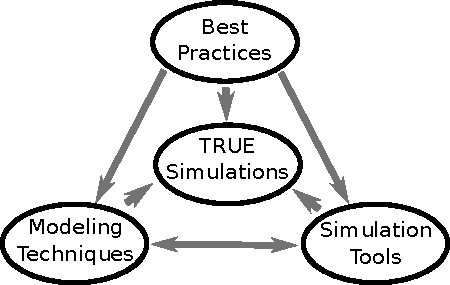
\includegraphics[width=3in]{figures/pub4/overview_2.pdf}
    \caption{
        Molecular simulations are becoming more informative and reproducible due to overlapping advances in modeling techniques and simulation tools through best practices in teaching, sharing, and software development.
    }\label{eco} %remember labels after caption, not before!
\end{figure}

``Best practices'' refers to the use of open software, software engineering practices, and pedagogy for teaching computing generally and molecular simulations specifically.
These practices have both a) enabled the creation of open source tools used broadly by the molecular simulation community, and b) been used within the molecular simulation community to advance simulation tools and modeling techniques (\autoref{eco}).
The ``simulation tools'' discussed are used primarily to perform molecular dynamics simulations using pairwise potentials to model the interactions between simulation elements.
Each of the main simulation engines is a significant feat of software engineering towards meeting their users' demands of application-specificity and performance.
``Modeling techniques'' refers to the algorithms used within simulation engines, interaction potentials (force fields), statistical sampling techniques, and theory. 
Explaining how practices, techniques, and engines are connected to each other is important because each area in isolation has near-infinite depth that can hinder accessibility to new researchers.

%%%%%%%%%%%%%%%%%%%%%%%%%%%%%%%%%%%%%%%%%%%%%%%%%%%%%%%%%%%%%%%%%%%%%%%%%%%%%%%%%%%%%
%%%%%%%%%%%%%%%%%%%%%%%%%%%%%%%%%%%%%%%%%%%%%%%%%%%%%%%%%%%%%%%%%%%%%%%%%%%%%%%%%%%%%
\section{Timescale problems}\label{s:timescale_problems}
Molecular simulations predict the structure and properties of materials using computer implementations of physics-based descriptions of matter.
The recent review article by Braun \textit{et al.} provides a comprehensive overview of the components and considerations for molecular dynamics (MD) simulations \cite{Braun2019}, which we also focus on here.
MD simulations suffer from two \textit{scaling} timescale problems: The more atoms needed to represent a system, (1) the more calculation time is required to generate the next configuration, and (2) the more configurations need to be sampled before equilibrium is achieved.
In other words, it takes a lot more time to simulate larger systems.
These timescale problems derive from algorithmic scaling of calculating interactions between $N$ simulation elements (often atoms) and because larger systems have more configurations (microstates) \cite{Frenkel2013,Miller2018}. 
Graphics processing units (GPUs) represent a major advance in computing hardware for ameliorating these scaling problems, and we recommend the 2010 review by Stone \textit{et al.} as a starting point \cite{Stone2010}. %
Because of the performance benefits of GPUs, all open-source MD packages now offer GPU support \cite{Anderson2008,Trott2011b,Anderson2013,Glaser2014b, Zheng2013}.

We introduce here the \textit{training} timescale problem that MD and MC simulation techniques also suffer from: 
Researchers spend more time making and fixing modeling errors as the number of software dependencies and scientific topics needed for the model increases, especially if any of them are new to the researcher.
The importance of the training timescale problem explains the growing efforts around training computational researchers \cite{Wilson2014c}.
Because scaling and training problems are obstacles to performing TRUE simulations, it is important for researchers to be mindful of tradeoffs between them when making modeling choices.

%%%%%%%%%%%%%%%%%%%%%%%%%%%%%%%%%%%%%%%%%%%%%%%%%%%%%%%%%%%%%%%%%%%%%%%%%%%%%%%%%%%%%
%%%%%%%%%%%%%%%%%%%%%%%%%%%%%%%%%%%%%%%%%%%%%%%%%%%%%%%%%%%%%%%%%%%%%%%%%%%%%%%%%%%%%
\section{Best practices and cognitive load}\label{s:practice}
Evidence-based instructional practices are being applied within communities of scientific software developers to create tools and training materials that feed back into these communities. 
Ambrose \textit{et al.} provides a comprehensive review of the science of teaching, and is an accessible introduction to research around \textit{cognitive load} that we focus on here \cite{Ambrose2010}. 
The basic idea of cognitive load is that the mental faculties of learners are finite, and their performance on a task (e.g., testing a new MD package) is hindered when they are asked to do more than one thing at a time \cite{Kahneman1973}.
The lens of cognitive load provides an accessible introduction to the research around stereotype threat and inclusivity, major barriers to participation of historically underrepresented groups in science, technology, engineering, and mathematics \cite{cheryan2009ambient,Shapiro2012,Schinske2016}.
Reduction of cognitive load is a principle of course design \cite{Bart2019,Cook2006,Simperler2015,Teal2015,Wilson2014,Foundation2016a}, human computer interactions \cite{Hollender2010}, model-based computing \cite{Bohner2010,Varga2014}, and efforts to make academic writing more accessible \cite{Oppenheimer2006}.
In particular, Software Carpentry, Data Carpentry, and Library Carpentry (\href{https://carpentries.org}{The Carpentries}) are community-driven projects that apply the science of teaching (especially cognitive load reduction) to empower individuals to use computing in support of their professions \cite{Wilson2014,Wilson2014c,Simperler2015,Teal2015,Foundation2016a}.
We focus on cognitive load because of its centrality to tool accessibility and inclusive research communities.

For a sense of the ubiquity of cognitive \textit{over}load in materials simulation, consider a novice simulator investigating how metal nanoparticles sinter on a surface during additive manufacturing in an atmosphere with alkanes.
They begin with an xml file and discover they need to use a command-prompt to get it ``in'' to their lab's simulation engine.
They review the literature to find dozens of seemingly appropriate forcefields with different parameterizations and functional forms \cite{Ponder2003}.
After selecting the embedded atom model \cite{Daw1983} to represent the metal atoms, they find difficulty choosing a forcefield for the atmosphere from  MM4 \cite{Allinger1996}, OPLS-AA \cite{Jorgensen1988}, GAFF \cite{Wang2004}, COMPASS \cite{Sun1998}, and TraPPE \cite{Keasler2012}, all with different models for the same compounds---how can this be? 
They consider the importance of charges, leading to Ewald summation \cite{Lebard2012} and polarizable force fields \cite{Halgren2001}.
They begin to despair and wonder if compiling a density functional theory package will be faster.
It isn't.
Now with six unresolved lines of questioning and a command-prompt that beeps at the letter `f', the simulator feels like they're moving backward.

Beeping prompts and sad students are finding help in the modern pedagogy summarized above, facilitated by the development of open-source tools.
It came as a surprise to many that large, decentralized software projects could be successful despite lack of private return \cite{Hippel2003}.
However, people enjoy helping each other online, both for the enjoyment of sharing their experiences and building professional reputation, and researchers further derive utility from software that helps with research \cite{Sarthou2005}.
This is apparent in the development logs of Carpentries lessons:
As one example, there are 1,942 commits from about 230 individuals since 2013, all attempting to make a better lesson for teaching the basics of version control (\href{https://github.com/swcarpentry/git-novice/commits/gh-pages}{Software Carpentry commit log}).
Open-source, GPU-accelerated MD engines have experienced growth in community development over the same time frame (\autoref{fig:commits}).
\begin{figure}
    \centering
    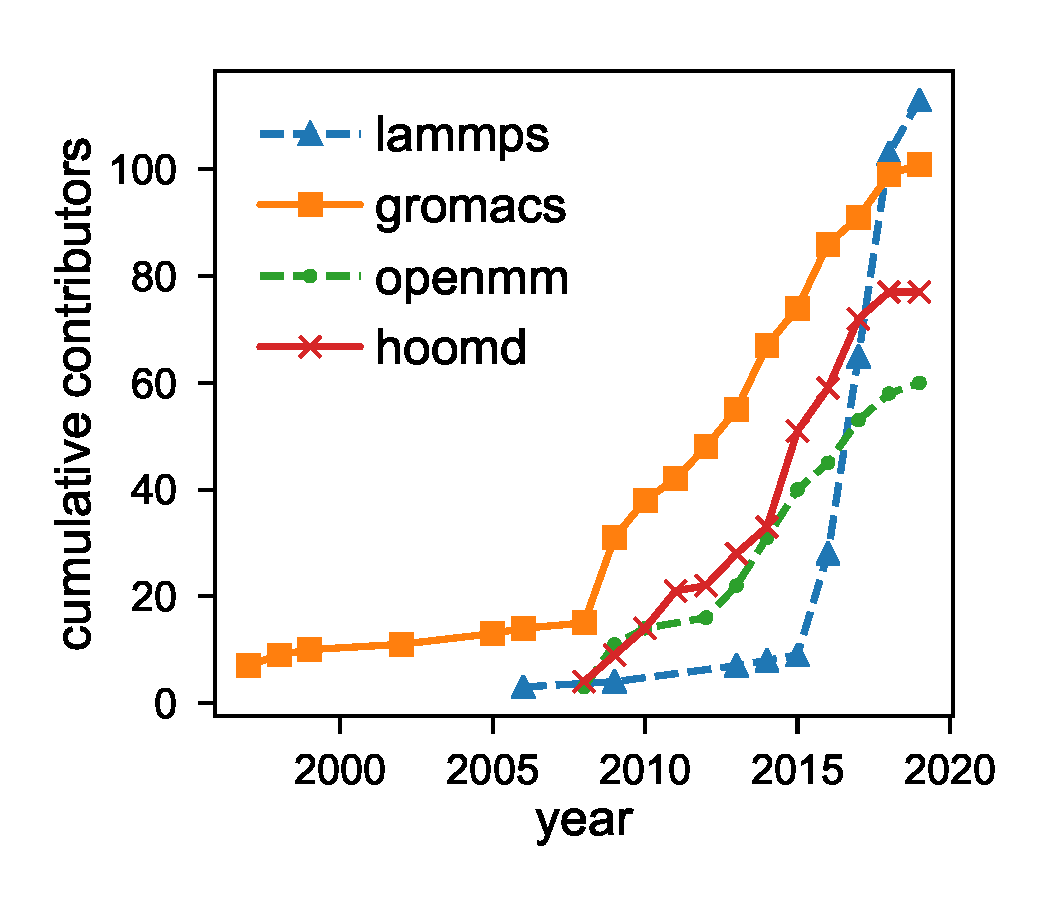
\includegraphics[width=3in]{figures/pub4/commits.pdf}
    \caption{Number of unique authors of four popular MD simulation engines over the last two decades. The increased growth around 2010 coincides with maturation of GPU technologies for MD and growth in Software Carpentry efforts. Numbers are approximate, as a few authors in each community may be double-counted if they commit with multiple pseudonyms.}\label{fig:commits}
\end{figure}
This is not to say any one of the Carpentries, GPUs, or GitHub explains the recent growth in open source science software, but instead emphasizes that coincident contributions to pedagogical practices, hardware advances, and online development communities are important in understanding this ecosystem.

Simulators are exchanging information beyond individual packages, now sharing teaching material under version control (\href{https://github.com/kofkeLab/Mol-Sim-Intro}{David Kofke's molecular simulation course}), pre-packaged virtual machines for workshops \cite{Jankowski2018b}, and new \href{https://www.livecomsjournal.org/}{journals } for living documents of best practices, tutorials, and perpetual reviews. %
A number of organizations have grown around the support of sustainable software development for science and the work of Katz \textit{et al.} provides a broad overview \cite{Katz2019}.
A list of tools for molecular simulation is included in \autoref{table:open-source-tools}, and \href{http://openscience.org/}{The OpenScience Project} catalogs hundreds of open projects across disciplines.

\begin{table*}
\caption{Open source software helpful for materials simulations.}
\centering
\begin{tabular}{|c|p{0.7\linewidth}|}
\hline
Package Name & Description  \\
\hline Diffractometer\cite{Jones2017, Diffract} & Python code for generating scattering patterns from MD snapshots  \\
\hline foyer\cite{Klein2018b} & Python package for atom-typing  \\
\hline freud\cite{Harper2016} & Python exposure of C++ analysis: RDF, order parameters, correlation functions   \\
\hline mBuild\cite{Klein2016mBuild} & Python package for system initialization with reusable, hierarchical components enabling complex initialization from simple building blocks \\
\hline MDAnalysis\cite{Gowers2016} & Python package for MD trajectory analysis supporting many file formats  \\
\hline MDTraj\cite{McGibbon2015} & Python package for analyzing and extracting information from MD trajectories  \\
\hline MorphCT\cite{Jones2017, MorphCT} & Python package for obtaining and aggregating charge transport properties from MD snapshots  \\
    \hline OVITO\cite{Stukowski2010} & Python explosure of C++ analysis: Visualization, structure determination \\
\hline packmol\cite{Martinez2009} & Library for initializing configurations of simulation elements\\
\hline physical\_validation\cite{Merz2018} & Python package for performing thermodynamic consistency checks \\ 
\hline Planckton\cite{planckton} & Python package for initializing and executing HOOMD-Blue (\texttt{hoomd}) simulations \\ 
\hline PLUMED\cite{Tribello2014} & Software for advanced sampling, using collective variables \\ 
\hline pyLAT\cite{Humbert2019} & Python package used to manage LAMMPS output \\
\hline Rhaco\cite{Rhaco} & Python package for initializing and simulating molecules and atoms at surfaces \\
\hline SSAGES\cite{Sidky2018} & Use collective variables and advanced sampling methods with amny engines \\
\hline signac-flow\cite{Adorf2018,signac_zenodo} & Python package for automating workflows including HPC schedulers and job submission \\
\hline signac\cite{Adorf2018,signac_zenodo} & Python package used to manage multi-dimensional data spaces and general workflows at scale  \\
\hline VMD\cite{Humphrey1996} & Interactive and scriptable visualize and analysis of simulations \\
\hline VOTCA\cite{Ruhle2009} & Package for automating coarse-graining and charge transport calculations \\
\hline
\end{tabular}
\label{table:open-source-tools}
\end{table*}

Beyond tools designed for molecular simulation, there are important categories of tools for lowering the cognitive load of software development and fostering collaboration.
\href{https://help.github.com/en/articles/applying-for-an-educator-or-researcher-discount}{GitHub}, 
\href{https://bitbucket.org/product/education}{Bitbucket}, 
and 
\href{https://about.gitlab.com/solutions/education/}{Gitlab} 
are the three largest platforms \cite{gitpopular} for collaborating on code repositories, and offer extra useful features at no cost for academic use. 
Messaging products Slack and Gitter are now popular for their integration with hosted repositories \cite{chatpopular} and lower the barrier to entry for discussing issues and getting help.
To lower the cognitive load of getting someone else's code to run, myBinder \cite{project_jupyter-proc-scipy-2018} enables users to launch Jupyter notebooks supporting multiple languages with pre-made enviroments for the code in question.
As examples, the \href{https://github.com/mosdef-hub/mosdef_tutorials}{MoSDeF tutorials}\cite{mosdeftut} use myBinder to spin up a Jupyter notebooks enabling users to begin tutorials without touching the software environment on their own computer. 
For solving the software stack problem on HPC clusters, singularity \cite{singularity2017} enables users to deploy portable ``containers'' from open-source Dockerfiles\cite{Merkel:2014:DLL:2600239.2600241} across multiple clusters, works with NVIDIA GPUS, and on many XSEDE resources.

Recurring themes in recommended readings \cite{Crick2015,Wilson2014,Katz2017} around best practices and considerations for community-driven scientific software development include:
\begin{enumerate}
    \item take into account cognitive load
    \item use version control
    \item automate repetitive tasks
    \item collaborate on and share open code
    \item write code in the highest-level language possible
    \item software development is a fundamental literacy for engineers and researchers.
\end{enumerate}
We also recommend Ref.~\cite{Gowers2016} as an example of a clearly described scientific software package (MDAnalysis) with relevance to materials simulation.

%%%%%%%%%%%%%%%%%%%%%%%%%%%%%%%%%%%%%%%%%%%%%%%%%%%%%%%%%%%%%%%%%%%%%%%%%%%%%%%%%%%%%
%%%%%%%%%%%%%%%%%%%%%%%%%%%%%%%%%%%%%%%%%%%%%%%%%%%%%%%%%%%%%%%%%%%%%%%%%%%%%%%%%%%%%
\section{Modeling Techniques}\label{techniques}
We now return to the original problem of advancing understanding of materials from molecular simulations and describe techniques for extracting more information from each step of an MD trajectory.
Both coarse-grained models and advanced sampling help with scaling timescale problems by focusing on the key features of the phenomenon of interest, spending less effort on irrelevant details.
In practice, implementing these techniques can lead to increased cognitive load if we are unaware of available infrastructure, so we organize key sources for learning more.

Briefly, by representing a collection of atoms with ``coarse'' simulation elements, significantly longer timescales are accessible because a) less computation is needed to compute the next configuration, and b) dynamics are accelerated because the underlying energy landscape is smoothed.
Simplified models of polymers are among the first systems studied with molecular simulations \cite{Richter1981,Kremer1990} and the literature around coarse-graining is now extensive.
For a polymer focus, see the recent perspective by Gartner and Jayaraman \cite{Gartner2019}.
For biomolecules and protein folding there are many good sources including the reviews of Voth \cite{Voth2008}, Clementi \cite{Clementi2008}, Elber \cite{Elber2005}, Klepeis \cite{Klepeis2009}, Kamerlin \cite{Kamerlin2011}, and Kmiecik \cite{Kmiecik2016}.
The MARTINI model stands out as a broadly successful coarse biomolecular model \cite{Marrink2014}.
The specific problem of virus capsid self-assembly is reviewed in Perlmutter \textit{et al.} \cite{Perlmutter2014}.
For multiscale modeling, coarse-grained potentials can be derived by matching structure \cite{Moore2014} or forces \cite{Lu2013,Wang2014j}, and the relative entropy framework of Shell and Chaimovich \cite{Shell2008,Chaimovich2010} provides a measure of information loss through coarse-graining. 

The calculation of free energy differences, rare events, and alternative approaches to sampling long dynamics can be accomplished by applying statistical mechanics to simulated trajectories.
SSAGES \cite{Sidky2018} provides a comprehensive overview of advanced sampling techniques as well as open software for deploying them.
Markov state models (MSM) \cite{Husic2018} are statistical tools for describing the coarse dynamics of MD trajectories and provide a way of aggregating information from multiple short runs.
MSMs themselves are a coarse-graining approach that has benefited from and contributed to the molecular simulation ecosystem. 
Machine learning approaches provide opportunities for extracting collective variables, trends, and patterns from materials simulations, and the review by Ferguson \cite{Ferguson2018} provides a current, comprehensive view.

%%%%%%%%%%%%%%%%%%%%%%%%%%%%%%%%%%%%%%%%%%%%%%%%%%%%%%%%%%%%%%%%%%%%%%%%%%%%%%%%%%%%%
%%%%%%%%%%%%%%%%%%%%%%%%%%%%%%%%%%%%%%%%%%%%%%%%%%%%%%%%%%%%%%%%%%%%%%%%%%%%%%%%%%%%%
\section{Organic photovoltaic structure and performance}\label{s:opv}
In this section we review key topics in simulations of organic photovoltaics (OPVs) and describe our recent work in this context.
OPVs convert photons into electrical current and engineering their structure to improve performance is an active area of research.
For a more detailed picture of why OPVs are a promising technology for sustainable energy generation, start with \cite{Espinosa2012,Mazzio2015}.
OPV performance is strongly dependent on the morphology, and Refs.~\cite{Vandewal2013,Clarke2010} provide overviews of the key factors governing charge generation, separation, and transport.
A review summarizing computational OPV morphology prediction at different length-scales is presented in Ref.~\cite{Harrelson2017}.
Computational predictions of OPV morphologies are used as inputs into charge transport simulations that link OPV structure to metrics determining their efficiency. 
Refs.~\cite{Clarke2010} and \cite{Groves2013b} explain charge generation and transport, while \cite{Groves2017a} explains how these properties can be simulated with kinetic Monte Carlo algorithms.
We summarize recent morphology and charge transport predictions of the benchmark OPV material poly(3-hexylthiophene) (P3HT) in \autoref{table:p3ht-simulations}.
Combining hardware, software, and coarse-graining advances, routine simulations of P3HT have improved by roughly four orders of magnitude over the last decade (0.6 monomer-$\mu$s in 2010 vs.~6900 monomer-$\mu$s in 2018). 

\begin{table*}
    \caption{Overview of recent computational studies of P3HT, including method (MD or MC), resolution (AA - all-atom, UA - united-atom, 3CG - coarse-grained with 3 simulation elements per repeat unit, 1CG - coarse-grained with one element per repeat unit), approximate number of repeat units simulated, simulation time, computational effort (estimated largest product of Repeats Units $\times$ Time), and if the structures were used for charge-transport calculations. 
    The work of Carrillo et al.\cite{Carrillo2013} is a notable outlier, having successfully combined coarse models of millions of repeat units with development access to the then-most-powerful supercomputer on the planet.
    *Explicit numbers were not provided in the report, but are estimated here.}
\centering
\begin{tabular}{|c|c|c|c|c|c|c|c|}
\hline
    Year & Study & Method & Model & Repeat Units & Simulation Time & Effort ($\mu$s)  & CT \\
\hline
    2010 & Moreno\cite{Moreno2010} & MD & AA & 300 & 2 ns & 6.0$\times 10^{-1}$  & No \\%More forcefield development
\hline
    2010 & Huang\cite{Huang2010} & MD & AA & 720 & 5 - 35 ns & 2.5$\times 10^{1}$  & No \\
\hline
    2010 & Huang\cite{Huang2010} & MD & 3CG & 36864 & 10 ns & 3.7$\times 10^{2}$  & No \\
\hline
    2011 & Lee\cite{Lee2011} & MD & 1CG & X & 10 ns & X  & No \\
\hline
    2013 & Bhatta\cite{Bhatta2013a} & MD & AA & 320-1280 & 5 ns & 6.4$\times 10^{0}$  & No \\%More forcefield development
\hline
    2013 & D'Avino\cite{DAvino2013} & MD & UA & 1600 & 60 ns & 9.6$\times 10^{0}$  & Yes \\
\hline
    2013 & Alexiadis\cite{Alexiadis2013} & MD & AA & 2700* & 20-45 ns & 1.2$\times 10^{2}$ & No \\
\hline
    2013 & Jankowski\cite{Jankowski2013} & MD & 3CG & 2250-3750 & 1.7 $\mu$s & 6.4$\times 10^{3}$  & No \\
\hline
    2013 & Carrillo\cite{Carrillo2013} & MD & 1CG & $3.2 \times 10^{6}$ & 400 ns & 1.3$\times 10^{6}$ & No \\
\hline
    2016 & Jones\cite{Jones2016} & MD & 3CG & 4600-17000* & 8 ns & 1.4$\times 10^{2}$  & Yes \\
\hline
    2016 & Scherer\cite{Scherer2016} & MD & 3CG & 8000 & 80 ns & 6.4$\times 10^{2}$  & No \\
\hline
    2017 & Jones\cite{Jones2017} & MD & 3CG & 2250-3750 & 1.7 $\mu$s & 6.4$\times 10^{3}$  & Yes \\
\hline
    2018 & Miller\cite{Miller2018, Miller2018a} & MD & UA & 1500-15000 & 0.3-3 $\mu$s & 6.9$\times 10^{3}$  & Yes \\
\hline
    2019 & Greco\cite{Greco2019} & MC & 1CG & 8000-16000 & N/A & N/A  & Yes \\
\hline
\end{tabular}
\label{table:p3ht-simulations}
\end{table*}

A challenge to making efficient OPVs is determining which combinations of photoactive compounds and thermodynamic conditions (temperature, pressure, concentrations) will result in a favorable morphology---a task well-suited to MD simulation.
Probing this vast data space requires organizing ensembles of simulations, distributing them on high-performance computing clusters, retrieving the data, and then distilling the data into understandable chunks.

In our recent work \cite{Miller2016,Henry2017a,Miller2018,Miller2018a}, we use HOOMD-Blue (\texttt{hoomd}) to predict morphologies of perylene, perylothiophene, P3HT, and poly(benzodithiophene-thienopyrrolo-dione) (BDT-TPD) oligomers using simplified (united atom) models.
Neglecting partial charges and treating conjugated systems as rigid are two assumptions that lower cognitive load associated with force fields, avoiding the first-principles calculation of unknown charge, dihedral, and angle parameterizations missing from OPLS-UA or GAFF.
These simplifications helped with both training and scaling timescale problems, resulting in morphology predictions in agreement with experiments \cite{Miller2016, Henry2017a,Miller2018} (see \autoref{p3htdiff} and \autoref{bdttpddiff}).

\begin{figure}
    \centering
    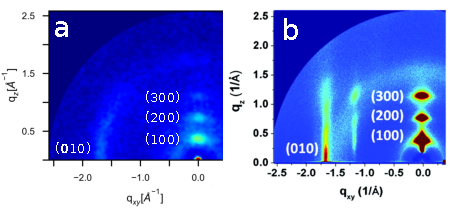
\includegraphics[width=3in]{{figures/pub4/diff_comparison}.pdf}
    \caption{
        a) Simulated and b) experimental grazing incident X-Ray scattering of P3HT show near identical features and wavenumbers along the (010) and (100) planes.
        The agreement indicates the same structures are being probed in both cases.
        Figure adapted with permission from Ref.~\cite{Miller2018}.
}
    \label{p3htdiff} %remember labels after caption, not before!
\end{figure}

\begin{figure}
    \centering
    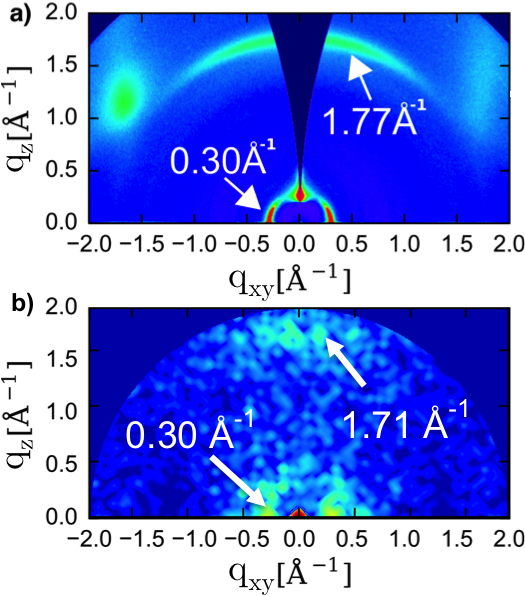
\includegraphics[width=3in]{figures/pub4/bdt_tpd_scattering.png}
    \caption{
        a) Experimental and b) simulated grazing incident X-Ray scattering of BDT-TPD showing agreement.
	The agreement validates our simplified model. 
	Reprinted with permission from\cite{Henry2017a}. Copyright 2017 American Chemical Society.
}
    \label{bdttpddiff} %remember labels after caption, not before!
\end{figure}

An example of developing transferable skills to deal with combinatorial explosion occured in this P3HT work: Only 14 temperatures, 6 solvent strengths, and 5 densities equates to 420 unique simulations.
In each of these 420 cases, we aim to understand how the proximity and orientation of thiophene rings  correlates with charge transport.
A single structural descriptor is applied to each case, and a ``phase-diagrams'' is constructed for each density, providing a handful of figures summarizing large data spaces (\autoref{p3ht}). 

\begin{figure} %
    \centering
    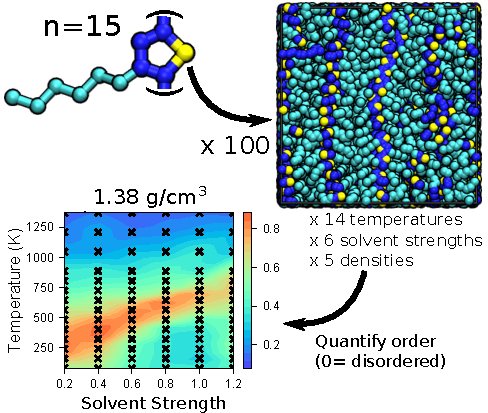
\includegraphics[width=3in]{{figures/pub4/p3ht}.pdf}
    \caption{
        100 P3HT chains of 15 repeat units are represented as three simulation species: Yellow (sulfur), blue (aromatic carbon), and cyan (aliphatic carbon).
Temperature, solvent strength (specified as a scaling of the Lennard-Jones well depth) and density, determine thermodynamic self-assembly of 420 unique structures.
    The self-assembled structures are quantified for ordering on the interval $[0, 1]$ - where 0 is completely disordered and 1 is completely ordered, according to the clustering of neighboring repeat units based on relative distances and orientations.
Ordering is then summarized into ``phase-diagrams'' depicting the order as a function of these three variables; demonstrating how hundreds of simulations can be distilled to a few, quickly interpretable figures.
}
    \label{p3ht} %remember labels after caption, not before!
\end{figure}

Testing transferability, reproducibility, usability, and extendibility of OPV modeling techniques is an exciting area of future work.
For P3HT in particular, the number of models, simulation engines, and sampling schemes used makes it a good candidate for evaluating TRUE-ness.
With a myriad of open approaches for coarse-graining, there is no fundamental reason why multiscale efforts validated by different groups could not be a test-bed for testing reproducibility these scales.
Similarly, the availability of various charge-transport calculation approaches provides for opportunities to reproduce predictions of how charge transport depends on morphology and chemistry.
Such cross-validation teams would help accelerate improvements around charge transfer calculations themselves, where opportunities exist to improve understanding of this broadly applicable phenomenon.

%%%%%%%%%%%%%%%%%%%%%%%%%%%%%%%%%%%%%%%%%%%%%%%%%%%%%%%%%%%%%%%%%%%%%%%%%%%%%%%%%%%%%
%%%%%%%%%%%%%%%%%%%%%%%%%%%%%%%%%%%%%%%%%%%%%%%%%%%%%%%%%%%%%%%%%%%%%%%%%%%%%%%%%%%%%
\section{Predicting crosslinking dynamics}\label{s:epoxy}
In this section we review computational approaches to predicting the crosslinked networks of toughened thermosets and discuss our recent work in this context.
Thermosets are strong, low-density materials formed by the covalent bonding of liquid precursors into a 3D network that can be made less brittle through the introduction of a thermoplastic ``toughener''. 
In the fabrication of composite materials made from carbon fibers impregnated with toughened thermosets the network is ``cured'' through the heating and cooling of a part over time.
The temperature history experienced by the part during curing influences the rates of diffusion and reaction, and therefore its resulting nanostructure and residual stresses.
As the thermoset precursors crosslink, there is an entropic driving force for the phase-separation of the thermoplastic \cite{Chen1999a}, which complicates nanostructure evolution.
For a review of the key concepts in modeling thermosets (cure fraction, gelation, and glass transition temperature) see Li and Strachan \cite{Li2015f}. 
The challenge focused on here is using molecular simulations to predict how thermoset formulation, toughener chemistry, and temperature history determine the cured nanostructure.

The central problems are those of scaling and training timescales, plus the fact that reacting systems are not in equilibrium.
On the sampling side, the slow dynamics of gelling, glassy thermosets make relaxation intractably long even for small systems.
Further, validating simulations against experimental systems with 1nm-100nm phase-separated length scales demands large simulated volumes. 
On the training side the main tensions are between faithful representation of reaction kinetics, coarse models that enable access to long timescales, and implementing these simultaneously.
The knowledge that the equilibrium integration schemes available in \texttt{hoomd} and \texttt{lammps} are in conflict with the exothermic formation of bonds, and that using ReaxFF \cite{VanDuin2001} won't permit sufficient volumes to be accessed is liberating:
It allows the question to be reframed as ``How predictive of nanostructure can a simplified model of crosslinking thermosets be?''

To advance towards the goal of large, fast, predictive thermoset simulations we develop \texttt{epoxpy} as detailed in Ref.~\cite{epoxpy}.
This was the first project in which we employed continuous integration into model development.
Sanity checks built around initialization of the tougheners and the generation of trajectories with and without the reaction algorithms implemented allowed the submission of large ensembles of jobs to multiple clusters with confidence. 
This further allowed the research team to quickly progress through a series of models in support of the science question:
\begin{itemize}
    \item DPD models are good for simplicity and performance, but not for representing entangled glasses
    \item LJ potentials and bond constraints can be parameterized to model entangled glasses
    \item Angle constraints are needed here for $T_g$ measurements to fit the DiBenedetto expression
    \item In some cases, million-particle systems are needed to capture the microphase separated morphologies (\autoref{epoxy_toc})
    \item Bond-forming models can be made with \texttt{hoomd} plugins and calibrated against reaction kinetic models with and without heats of reaction
\end{itemize}
The results of our approach are summarized with recent simulations in~\autoref{table:DGEBA_DDS_PES_model_comparison}.
The two distinguishing features of our recent work (\cite{epoxpy}) are (1) the ability to investigate structural evolution while the model epoxies cure and (2) ability to do so for million-particle volumes in a few days or weeks on a single GPU.

\begin{table}
\caption{Overview of recent reacting epoxy models, sorted by system size. Most efforts do not capture dynamic bonding during MD integration nor validate glass transition ($T_g$) as a function of cure fraction $\alpha$ (DiBenedetto expression).}
\label{table:DGEBA_DDS_PES_model_comparison}
\centering
\begin{tabular}{|c|c|c|c|}
\toprule
\thead{Model\\(Chemistry)} & \thead{Bond \\Probability} & \thead{System Size} & \thead{$T_g(\alpha)$ \\Validation} \\ \midrule
    \thead{CGMD\cite{Komarov2007a}\\EP/CA} & \thead{Arbitary}& $5.0\times10^{3}$ & No\\
\thead{AAMD\cite{Gissinger2017} \\(DGEBA/DETA)} & \thead{Arbitary}& $5.9\times10^{3}$& No \\
\thead{CGMD/AAMD\cite{Langeloth2015} \\(DGEBA/DETA)} & \thead{1}& $2.2\times10^{4}$& No\\%$0.4$ \\
\thead{AAMD\cite{Li2012n} \\(DGEBA/33DDS)} & \thead{1}& $6.9\times10^{4}$& No \\
\thead{AAMD\cite{Khare2018} \\(DGEBA/44DDS)} & \thead{1}& $9.8\times10^{4}$& No  \\
\thead{DPD\cite{Kacar2015} \\(DGEBA/DETA)} & \thead{1}& $1.1\times10^{5}$& No  \\
\thead{DPD\cite{Liu2011g} \\(DDS/RA/SA)} & \thead{0.001}& $2.5\times10^{5}$& No \\
\thead{CGMD/DPD\cite{thomas2018new}\\(DGEBA/44DDS/PES)} & \thead{$\sim\exp(\frac{E_a}{k_BT})$} & $4.0\times10^{6}$& Yes\\%$0.4,1.0$ \\
\bottomrule
\end{tabular}
\end{table}

\begin{figure}
    \centering
    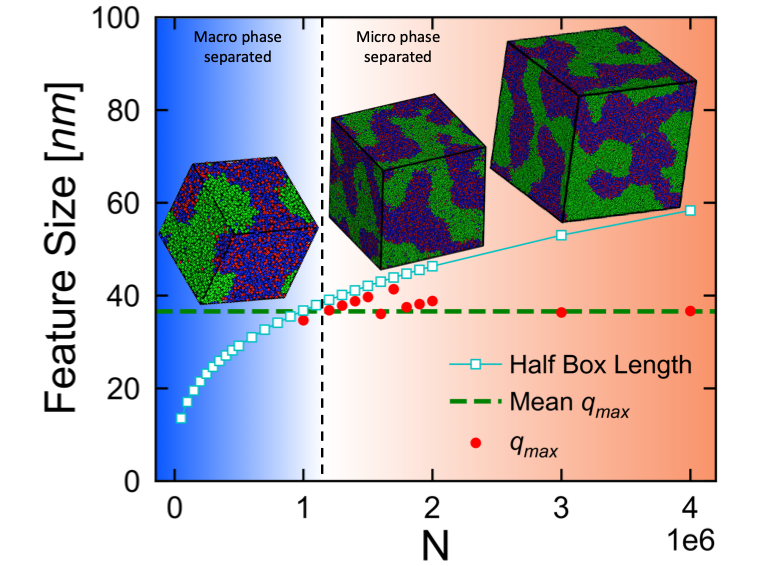
\includegraphics[width=3in]{figures/pub4/epoxy_toc.png}
    \caption{The ability to perform curing simulations of million-particle toughened thermoset models enables the identification of sufficient box sizes. Here, divergence of the low-wavenumber structure factor is used to identify macrophase separation, and for small volumes (blue, left) of this CG model the morphologies appear macrophase separated. Large volumes (orange, right) of the same model show a local maximum in the structure factor ($q_{max}$) indicating microphase separation is observable when the length-scales of separation are smaller than half the simulation box length. Here, 1.2e6 particles (35nm boxes) are needed, reinforcing the importance of fast, large simulations for studying toughened epoxy thermosets.
    %permission info below
   %Title of the Work, Author (s) and/or Editor(s) Name (s), Title of the Journal, Vol and Issue No., Copyright @ year and name of the publisher 
    }
    \label{epoxy_toc} %remember labels after caption, not before!
\end{figure}

Despite the simplifications, our coarse simulations match experimental reaction dynamics and glass transition temperatures \cite{thomas2018new}.
Further, because we can vary temperature over the course of these reacting systems we can for the first time use MD to investigate how nanostructure depends upon temperature history during curing.
Here we present new results (\autoref{epoxy_pre_gel} and \autoref{epoxy_post_gel}) summarizing the evolution of structure in two types of curing simulations where the primary activation energy is 2.1 dimensionless energy units, the secondary $E_A=2.52$, $N=400000$, $L=73.7$nm and $dt=0.01$, using the Lennard-Jones parameters from Table 5.1 and the fiducial simulation parameters from  table 5.2 of~\cite{thomas2018new}.
Specifically, the ratio of coarse amine, epoxy, and toughener (A, B, and C) considered here is 1:2:2, with $\varepsilon_{AA}=0.9216, \varepsilon_{BB}=1.0, \varepsilon_{CC}=0.8840$, $\varepsilon_{AB,AC,BC}$ are obtained using the Lorentz-Berthelot mixing rule (e.g. $\varepsilon_{AB}=\sqrt{\varepsilon_{AA}\varepsilon_{BB}}$), harmonic bond $r_0=1.0$ and $k=100 \frac{\varepsilon}{\sigma^2}$. %, angle constraint $\theta_0=109.5$  and $k_\theta=25 \frac{\varepsilon}{\theta^2}$.
The Langevin thermostat with drag parameter $\gamma=4.5$ is used to advance simulation trajectories.
Simulations were performed on NVIDIA K40 cards using hoomd 2.2.1 (commit hash f664aebdf55e44f10cdd6d5edc3a090f1bca713b), 

In both figures, the wavenumber associated with microphase separation is plotted vs.~time, with the simulation temperature (red) overlaid, along with the system's glass transition temperature (purple) which is a function of the degree-of-cure. 
In \autoref{epoxy_pre_gel}, the sample being cured at 0.8 kT (above $T_g$) is quenched to 0.5 kT (below $T_g$) before gelation, and in \autoref{epoxy_post_gel} the quench occurs after the onset of gelation. 
In both cases, the morphologies achieve the same degree of cure ($\alpha=0.78$), and the standard error of five independent simulations are plotted with the grey error bars. 
We observe that curing post-gelation narrows the variance in cured structure, and these results demonstrate the importance of temperature history on cured morphology.

\begin{figure}
    \centering
    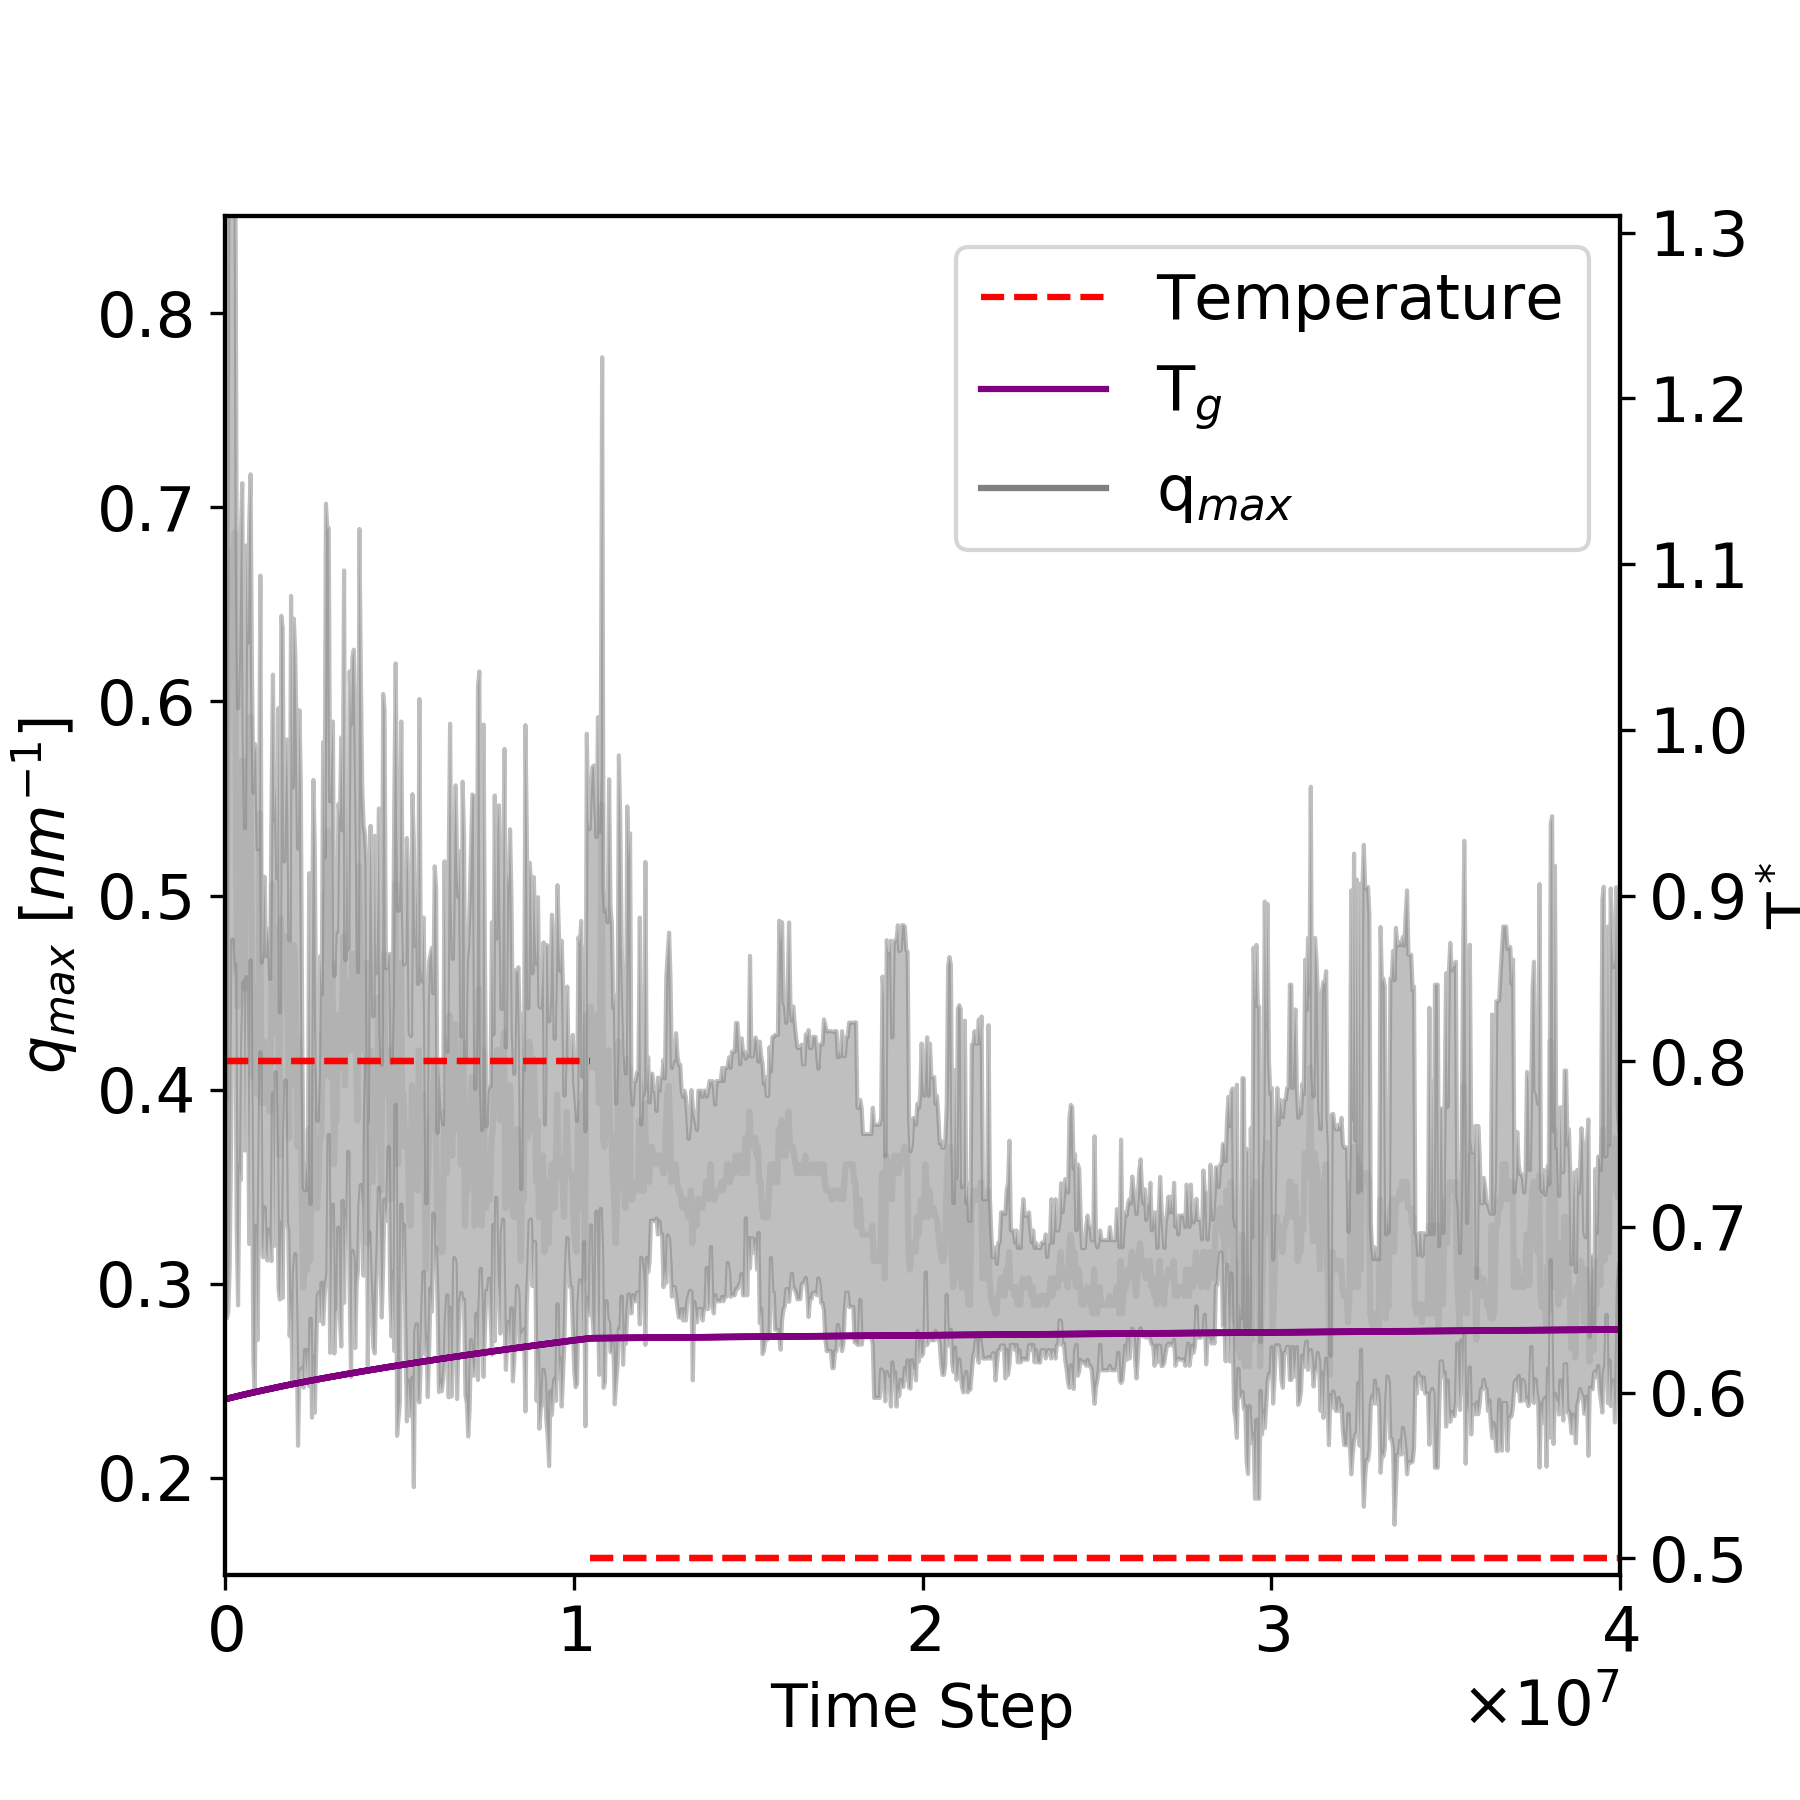
\includegraphics[width=3in]{figures/pub4/epoxy_pre_gel.png}
    \caption{Time evolution of the dominant length scale measured by the toughener-toughener structure factor for toughened reacting epoxy thermosets quenched below $T_g$ (solid line) before gelation at time step 10,480,000. Curing temperature is shown by the dotted line. Error bars represent standard error from five independent simulations}
    \label{epoxy_pre_gel} %remember labels after caption, not before!
\end{figure}

\begin{figure}
    \centering
    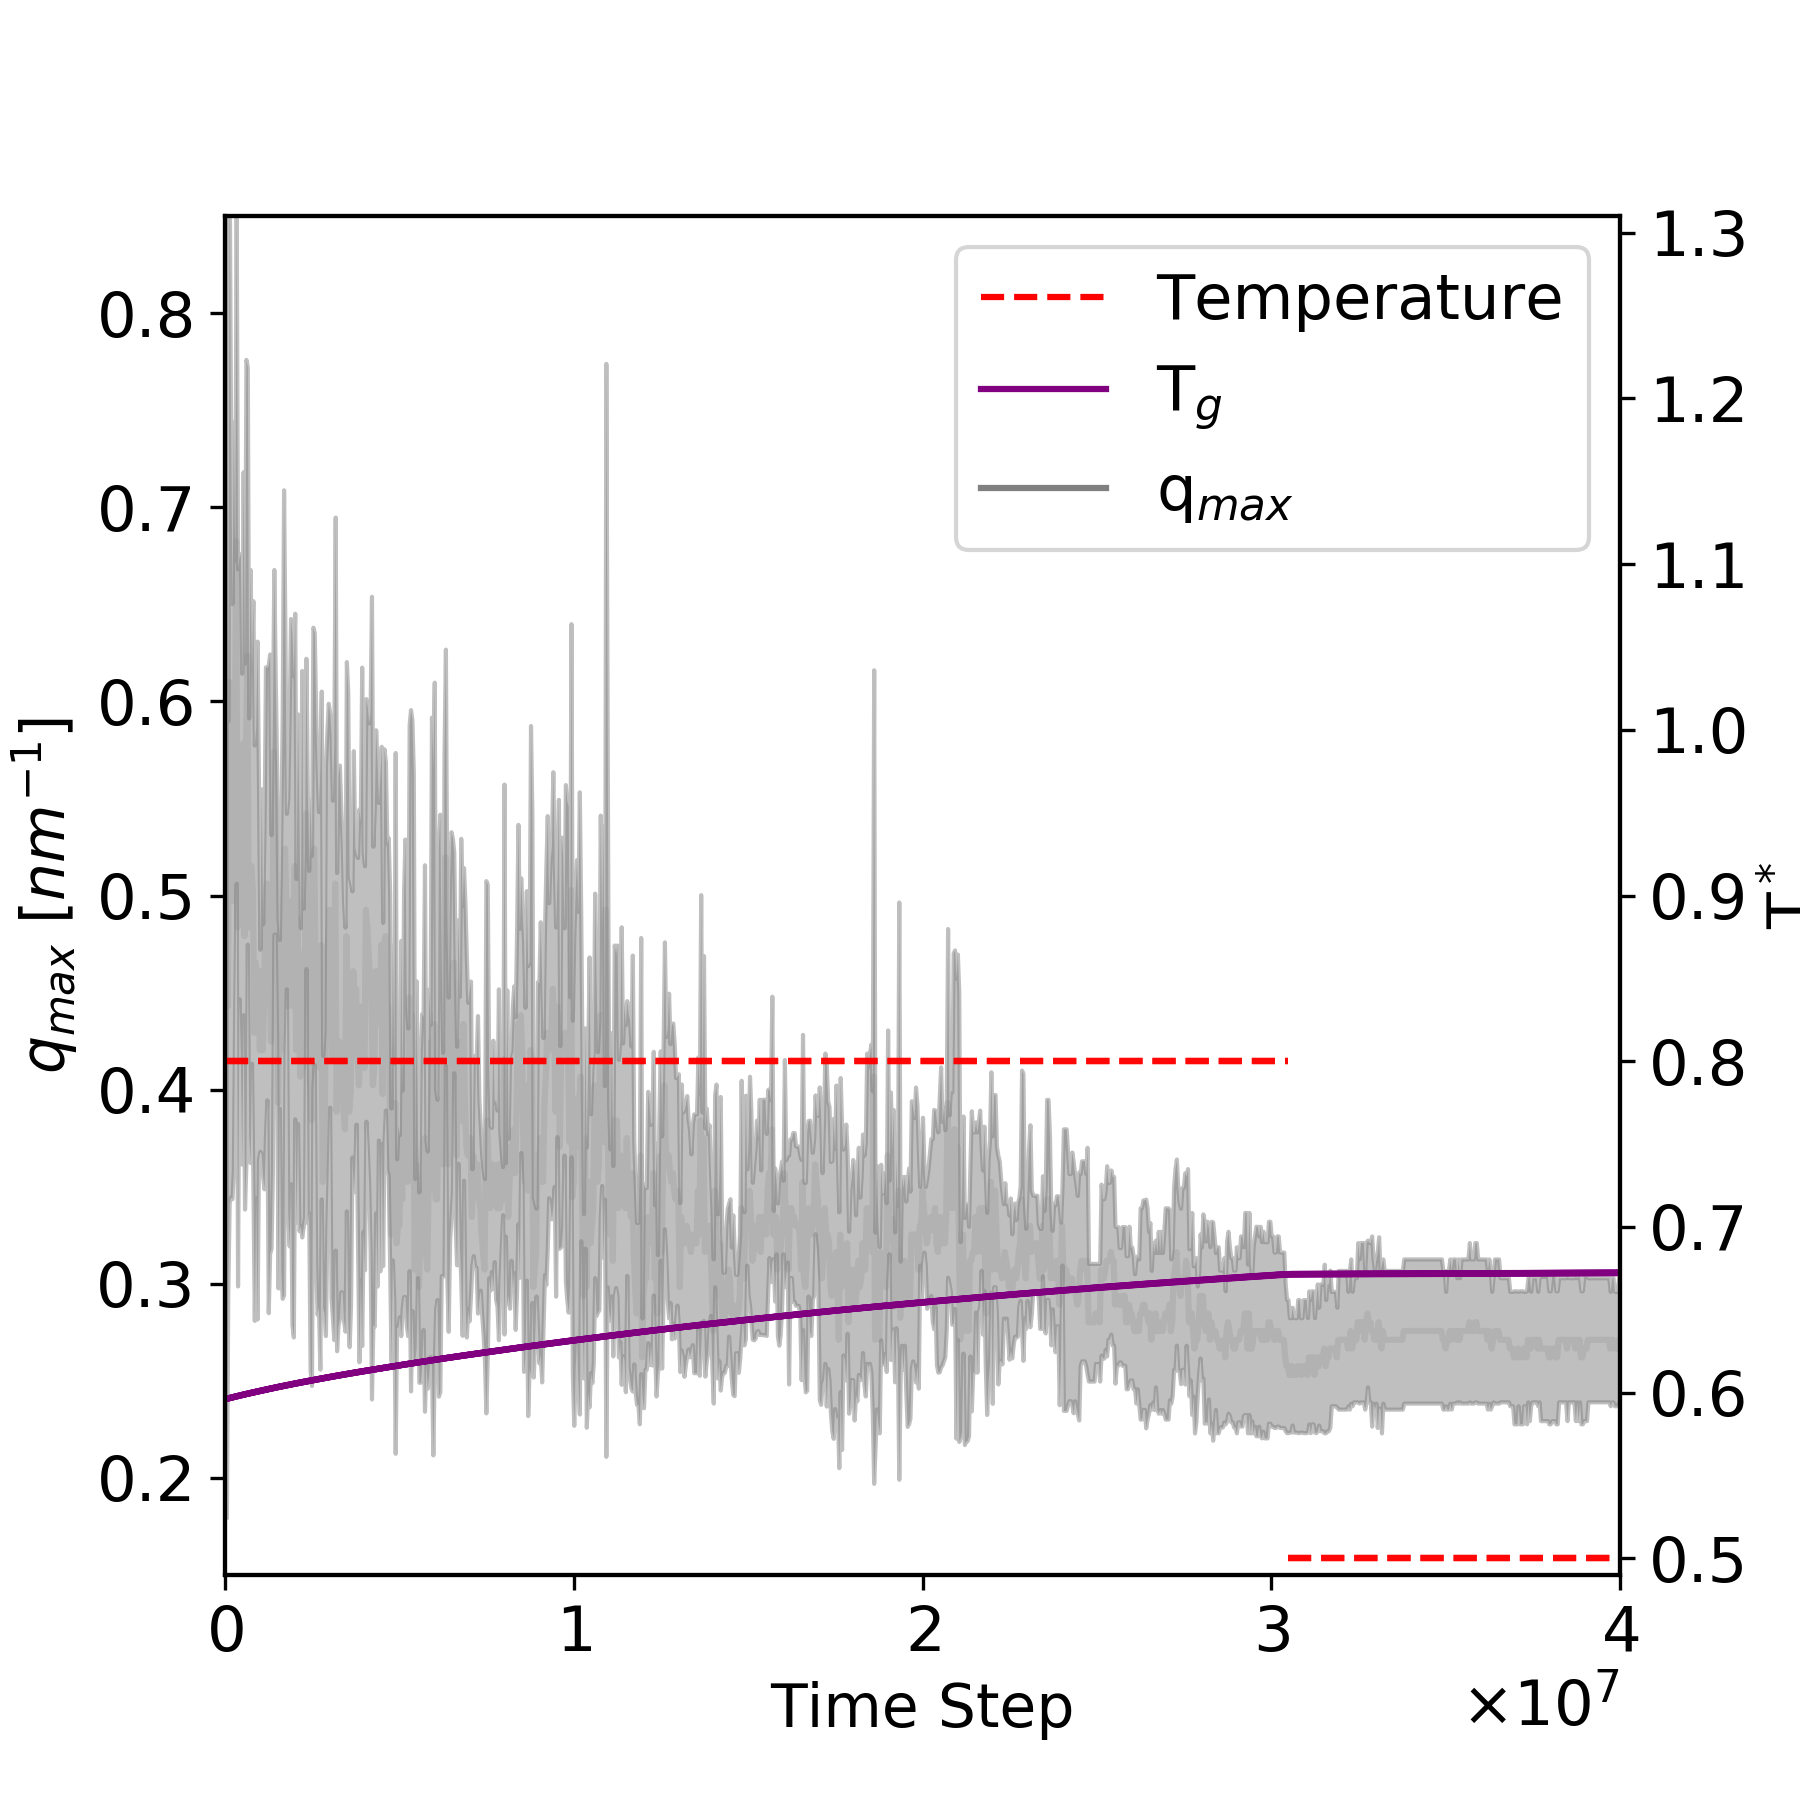
\includegraphics[width=3in]{figures/pub4/epoxy_post_gel.png}
    \caption{Time evolution of the dominant length scale measured by the toughener-toughener structure factor for toughened reacting epoxy thermosets quenched below $T_g$ (solid line) after gelation at time step 30,480,000. Curing temperature is shown by the dotted line. Error bars represent standard error from five independent simulations}
    \label{epoxy_post_gel} %remember labels after caption, not before!
\end{figure}

The present example combining simplified models with continuous integration---two of the best practices from \autoref{s:practice}---demonstrates improved understanding of materials behavior.
Because the code is open, the data is available, and because experimentation in this area is active, we identify epoxy thermosets as an area where we expect development around TRUE simulations to accelerate.
Community validation of morphology predictions from simulations with varied temperature histories offers opportunity to increase the industrial impact of molecular simulations.

%%%%%%%%%%%%%%%%%%%%%%%%%%%%%%%%%%%%%%%%%%%%%%%%%%%%%%%%%%%%%%%%%%%%%%%%%%%%%%%%%%%%%
%%%%%%%%%%%%%%%%%%%%%%%%%%%%%%%%%%%%%%%%%%%%%%%%%%%%%%%%%%%%%%%%%%%%%%%%%%%%%%%%%%%%%
\section{Training new simulators}\label{s:train}
In this section we describe several examples of on-boarding students to new projects wherein open tools (namely \texttt{hoomd}, mBuild, foyer, signac) and Software Carpentry pedagogy are used to reduce cognitive load and aid reproducibility.
In addition to using the aforementioned tools directly in python scripts, we develop two packages, Rhaco \cite{Rhaco} and Planckton \cite{planckton}, that combine these tools to accomplish common tasks for specific systems.
Rhaco facilitates the initialization and simulation of matter near surfaces and Planckton provides infrastructure for coupling MD simulations of OPVs to charge transport simulations (\autoref{table:open-source-tools}).
Examples of the diverse surface systems investigated with Rhaco are summarized in \autoref{fig:rhaco} and have enabled broad testing of forcefield compatibilities and qualitative investigation of surface phenomena while teaching students from multiple disciplines.
In \autoref{fig:mbuild} we summarize DNA, fullerene, OPV material, asphaltene, and patchy particle models developed by new students leveraging mBuild and \texttt{hoomd}. 
\begin{figure}
    \centering
    \includegraphics[width=6in]{figures/pub4/rhaco.pdf}
    \caption{a) PDMS chains initialized over NiMnGa, b) configuration of PDMS on NiMnGa by combining UFF and an OPLS-UA-derived potential, c) PDMS initialized on an M1 surface, d) Sintering silver nanoparticles on a corundrum surface combining EAM and UFF.}\label{fig:rhaco} %remember labels after caption, not before!
\end{figure}
These examples are representative of students being able to initialize and debug models in weeks.
In the case of \autoref{fig:mbuild}a, quickly moving past the initialization step of building coarse-grained DNA identified issues with our implementation of the Knotts model.
In \autoref{fig:mbuild}b, the minimal physics for polar fullerene oxides solubilizing C$_{60}$was identified by trying seven coarse models. 
In \autoref{fig:mbuild}c, initializing the complex truxene (a new candidate molecule for OPVs) with foyer immediately identified needed dihedral constraints.
The asphaltenes components in \autoref{fig:mbuild}d can be tuned for molecular weights and number of chains and was accomplished by an REU team.
The patchy trapezoids in \autoref{fig:mbuild}e permit quick testing of how patch size and shape influences assembly propensity.
\begin{figure}
    \centering
    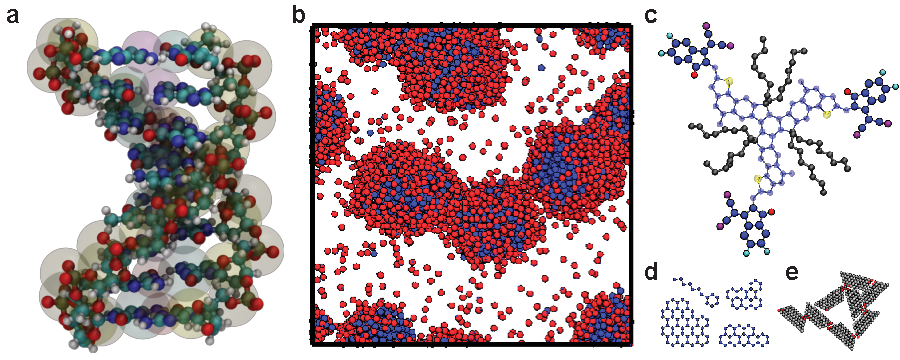
\includegraphics[width=6in]{figures/pub4/mBuild.pdf}
    \caption{a) Coarse-grained DNA initialized directly from sequence of nucleobases using the model from \cite{Knotts2007}, b) Micelle self-assembly from a coarse-grained model of fullerene and their oxides, c) truxene molecule with electroactive components core and three functional groups, d) examples of programmatically-generated asphaltene components, e) 2D patchy particles designed to self-assemble terminal structures.}\label{fig:mbuild} %remember labels after caption, not before!
\end{figure}

By combining tools for particular applications, we create ``higher-level'' languages for describing the system initializations in these examples.
This enables the concepts of the models to be probed faster, lowering the load associated with initialization and parameterization, and the management of conversion between units and dimensionless quantities used in \texttt{hoomd}. 
Further, the code development benefits are bidirectional: By engaging with developer communities, students broaden their network of support and provide feedback that informs tool development.
All of the repositories mentioned here (\texttt{hoomd}, mBuild, foyer, signac, and Software Carpentry's instructor training) have now merged student pull requests originating from missing features or bugs encountered en route to the above work.
These examples dispel the notion that aiming for simplicity necessarily creates ``black-boxes'' that limit student understanding of details, or the notion that higher-level languages necessarily create dependencies on established techniques.
Rather, aiming for low cognitive load can focus development of new techniques and features with the best payoff for the researcher.
Students anecdotally report increased interest and confidence, and this area represents a potential opportunity for future studies of professional identity, retention, and long-term career outcomes \cite{Ibarra1999}.

Related to the professional identities of materials simulators is the idea that certain scientist roles might enhance TRUE simulations.
For example, should training prioritize the development of tool developers and tool users separately, or jack-of-all-trades scientists that can do everything?
We find guidance to answering this question from our experiences with distributed code development: 
It is impossible for any individual to master everything, so leveraging the knowledge embedded in diverse development communities should be prioritized.
Prioritizing diverse development communities highlights the need for the individuals in these communities to communicate and collaborate.
The existence of and adherence to community codes of conduct (see The Carpentries \href{https://docs.carpentries.org/topic_folders/policies/code-of-conduct.html}{code of conduct}, for example) helps to ensure communities practice inclusivity and fosters collaboration.
Within such communities we do not know if the prioritization of particular roles is yet warranted to enhance the realization of TRUE simulations, but we hold the optimistic opinion that communities offer the opportunity for the ensemble of individual interests and strengths to overlap in a way that makes any individual's shortcomings irrelevant.

%%%%%%%%%%%%%%%%%%%%%%%%%%%%%%%%%%%%%%%%%%%%%%%%%%%%%%%%%%%%%%%%%%%%%%%%%%%%%%%%%%%%%
%%%%%%%%%%%%%%%%%%%%%%%%%%%%%%%%%%%%%%%%%%%%%%%%%%%%%%%%%%%%%%%%%%%%%%%%%%%%%%%%%%%%%
\section{Outlook}
This instant in time represents a period of major change in the materials simulation ecosystem.
Distributed coding communities have appeared, grown (\autoref{fig:commits}), and disrupted the development practices and availability of simulation tools, continuing progress towards TRUE simulations since the field's origins \cite{Metropolis1953,Alder1957}.
In this perspective we make the case for thoughtful training to take a central role in enhancing research reproducibility while simultaneously training researchers for broadly-needed technical roles. 
We also make the case that \textit{en route} to TRUE simulations, these simulations should begin as less ``true'': Lowering cognitive load by sacrificing completeness now is made up for by increased efficiency and correctness later.
However, TRUE simulations are not yet the norm.
Materials simulators are in a position of opportunity and responsibility: We can demonstrate how reproducible science can be performed through increased engagement with our peers in the coming years.
If the current momentum around communication and collaboration wanes, however; if the community becomes less inclusive rather than more, we may expect the amount of beeping prompts to increase.
We take a more optimistic view: There has never been a better time to be a molecular simulator because of how active the community is with helping train its members to do transferable, reproducible, usable, extensible science. 

%%%%%%%%%%%%%%%%%%%%%%%%%%%%%%%%%%%%%%%%%%%%%%%%%%%%%%%%%%%%%%%%%%%%%%%%%%%%%%%%%%%%%
%%%%%%%%%%%%%%%%%%%%%%%%%%%%%%%%%%%%%%%%%%%%%%%%%%%%%%%%%%%%%%%%%%%%%%%%%%%%%%%%%%%%%
\section{Acknowledgements}
\label{ack}
This material is based upon work supported by the National Science Foundation under Grants No. 1835593, 1653954, 1658076, and 1229709.
This work used the Extreme Science and Engineering Discovery Environment (XSEDE), which is supported by National Science Foundation grant number ACI-1053575 \cite{Towns2014}.
This research is part of the Blue Waters sustained-petascale computing project, which is supported by the National Science Foundation (awards OCI-0725070 and ACI-1238993) and the state of Illinois. 
The authors gratefully acknowledge sponsorship through the Laboratory Directed Research and Development (LDRD) program of the Idaho National Laboratory.
This material is based upon work supported by The Boeing Company under contract BRT-LO118-0015.
We acknowledge high-performance computing support of the R2 compute cluster (DOI: 10.18122/B2S41H) provided by Boise State University's Research Computing Department.
Blue Waters is a joint effort of the University of Illinois at Urbana-Champaign and its National Center for Supercomputing Applications. 
KN, BA, MA, JG and EJ thank the Shodor Education Foundation and the Blue Waters Student Internship Program for support of this work. 

The raw and processed data required to reproduce these findings are available to download from \href{https://doi.org/10.5281/zenodo.2619585}{https://doi.org/10.5281/zenodo.2619585}. 
